\documentclass[twocolumn]{article}
\usepackage{graphicx}
\usepackage{amsmath}
\usepackage[colorlinks=true, allcolors=blue]{hyperref}
\usepackage{float}
\usepackage{geometry}
\usepackage[sorting=none]{biblatex}
\usepackage{ragged2e} 
\usepackage{xurl} 

\geometry{top=2cm, bottom=2cm, left=3cm, right=2cm}

\addbibresource{references.bib} 

\begin{document}

\begin{titlepage}
    \centering
    \vspace*{1cm}
    
    {\LARGE \bfseries Department of Information and Communication Technology \par}

    \begin{figure}[H]
        \centering
        \includegraphics[width=0.75\linewidth]{logo.png}
    \end{figure}
    
    \vspace{1cm}
    
    {\Huge \bfseries Machine Learning in Medicine \par}
    
    \vspace{1cm}
    
    {\Large Breast Cancer Binary Classification \par}

    \vspace{2cm}
    
    {\large \textbf{Group 3} \par}
    \vspace{0.5cm}
    {\large 
        22BI13387 - Trinh Van Quyet\\
        22BI13067 - Nguyen Tien Cong\\
        22BI13103 - Le Duc Dung\\
        22BI13233 - Tran Tuan Kiet\\
        22BI13280 - Do Duy Minh \\
    \par}

    \vspace{1.5cm}
    
    {\large \textbf{Lecturer:} Assoc.Prof. Tran Giang Son \par}
    
    \vspace{1.5cm}
    
    {\large Academic year: 2022 - 2025} \par
    
    \vspace{0.5cm}
    
    {March 6, 2025}
    
\end{titlepage}

\onecolumn
\tableofcontents
\newpage       

\twocolumn
\begin{abstract}
    Breast cancer is one of the leading causes of cancer-related deaths worldwide, highlighting the importance of accurate and efficient diagnostic tools. The BreakHis (Breast Cancer Histopathological) dataset \cite{Spanhol2016} \cite{BreakHis2016} provides a comprehensive collection of 9,109 histopathological images of breast tumors, enabling advancements in automated tumor classification through machine learning. Collected from 82 patients, the dataset is divided into benign (2,480 images) and malignant (5,429 images) categories, with images captured at varying magnifications (40X, 100X, 200X, and 400X).
    
    This report explores the potential of the BreakHis dataset in aiding the development of ViT-based models for binary class of tumor classification. This method will provide a way for more effective breast cancer diagnosis and treatment strategies.
\end{abstract}
\addcontentsline{toc}{section}{Abstract}

\section{Introduction} 
\subsection{Context}
Breast cancer remains a significant global health challenge, ranking as one of the most prevalent cancers among women worldwide. Early and accurate diagnosis plays an important role in improving patient outcomes and survival rates. Traditional diagnostic methods, such as manual histopathological examination, are often time-consuming and subject to inter-observer variability. 

\subsection{Objective}
In recent years, the application of machine learning (ML) and computer vision techniques has shown immense promise in automating and enhancing the accuracy of breast cancer diagnosis. This report focuses on leveraging the BreakHis dataset to develop Vision Transformer (ViT) based models for the binary classification of breast tumors.

\section{Methodology}
\subsection{Data Exploration}
The BreakHis - Breast Cancer Histopathological Dataset is a valuable resource for medical image analysis, particularly in the classification of breast cancer. This dataset contains high-resolution histopathological images of breast tissue, divided into both binary and multi-class labels, to support the development and evaluation of machine learning models in cancer classification.

The dataset has two classification types: binary classification (Benign vs. Malignant) and multiclass classification (8 different tumor types). But in this report, we will concentrate on the binary classification.

This dataset also contains four magnification levels: Images are available at 40X, 100X, 200X, and 400X magnifications, allowing models to learn across varying levels of tissue detail.

\begin{figure}[H]
    \centering
    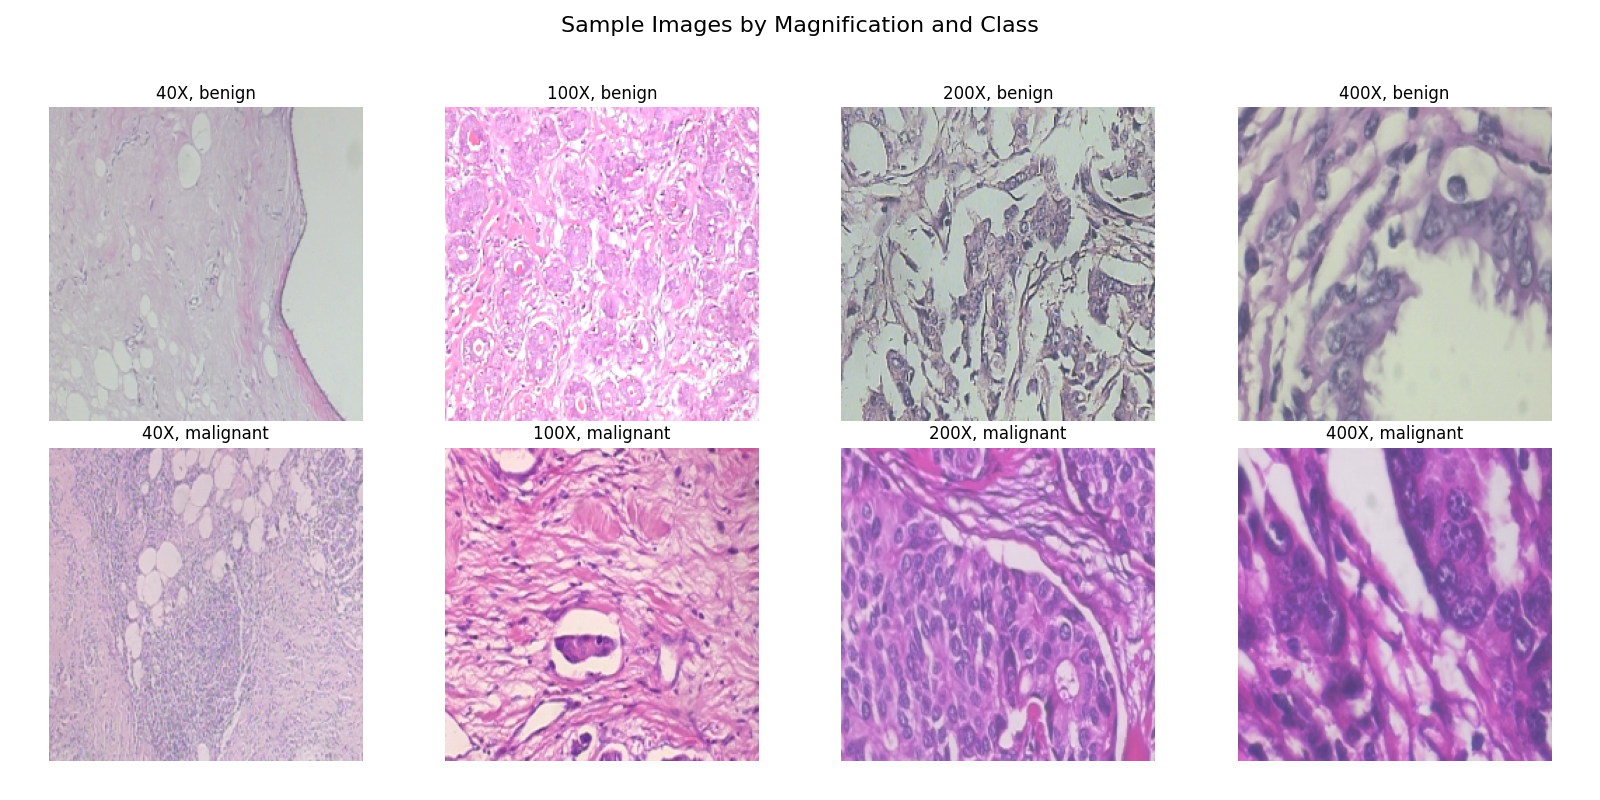
\includegraphics[width=1\linewidth]{sapmle.png}
    \caption{Samples by Magnification}
    \label{fig:enter-label}
\end{figure}

This BreakHis dataset is significantly imbalanced with 2480 samples in benign class and 5429 samples in malignant class.

\begin{figure}[H]
    \centering
    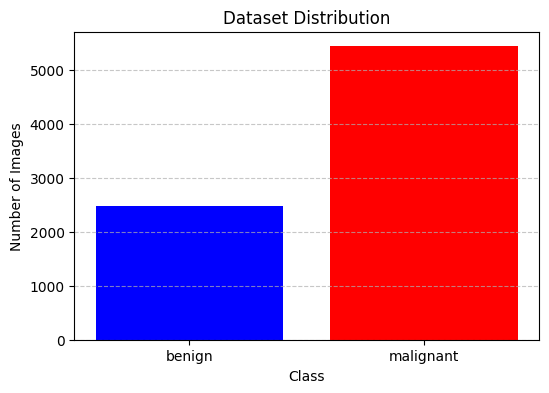
\includegraphics[width=1\linewidth]{distribution.png}
    \caption{Class Distribution}
    \label{fig:enter-label}
\end{figure}

\subsection{Data Preprocessing}
\subsubsection{Contrast Enhancement}
In this section, we apply CLAHE (Contrast Limited Adaptive Histogram Equalization) to improve visibility for a better feature extraction process.

\begin{figure}[H]
    \centering
    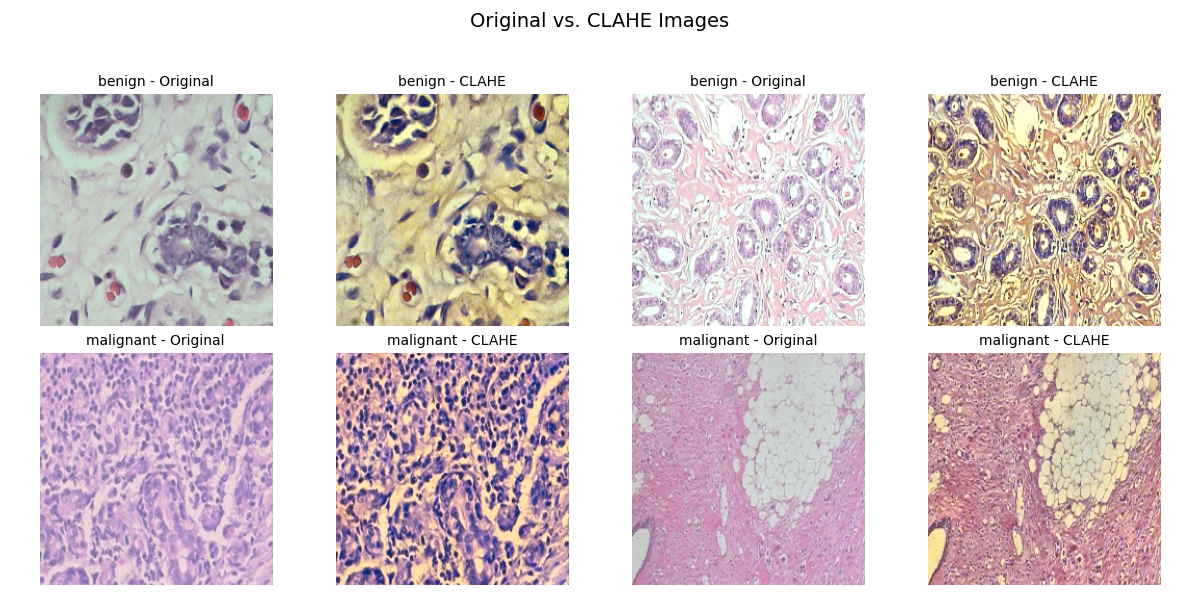
\includegraphics[width=1\linewidth]{clahe.png}
    \caption{Original vs. Enhanced Samples}
    \label{fig:enter-label}
\end{figure}

The RGB images are converted to the LAB color spaces:
\begin{itemize}
    \item L: Brightness (Lightness)
    \item A: Green–Red component
    \item B: Blue-Yellow component
\end{itemize}

We applied CLAHE on the L channel to improve overall contrast and on the B channel to increase the visibility of details. As the result, samples are refined local contrast without over-saturating, with enhanced details in dark and bright areas, reduced overexposure in high-intensity regions and preserved natural colors by modifying only the Lightness and Blue-Yellow channels.

\subsubsection{Tokenization}
Before tokenization, images are preprocessed to ensure consistency in size, format, and normalization. The following transformations are applied:
The RGB images are converted to the LAB color spaces:
\begin{itemize}
    \item Resize: Reshape all images to a fixed size of 224x224 pixels.
    \item Random Horizontal Flip: Augment data by flipping images horizontally.
    \item Convert to Tensor: Transform images into numerical tensor format.
    \item Normalize: Adjust pixel values based on ImageNet\cite{imagenet_cvpr09} mean and standard deviation to stabilize training.
\end{itemize}

Then a pre-trained image processor for ViT based\cite{dosovitskiy2020image} from Hugging Face\cite{HugginFace} is used to handle image tokenization. The processor extracts pixel values and formats them into tensors for the model. The tokenization function is applied to the entire dataset to convert all images into a format suitable for the model.

\subsection{Model}
We decide to approach this task by fine-tuning the ViT model with LoRA (Low Rank Adaptation)\cite{hu2022lora}. In LoRA (Low-Rank Adaptation), we apply trainable low-rank modifications to specific attention layers of a pre-trained model. The Query (Q) and Value(V) layers get adjusted because of their importance for computing self-attention, which determines how different image patches relate to each other. Modifying only the Query and Value layers reduces the number of trainable parameters while still allowing the model to learn new representations. The choice of adaptation on these layers is critical for efficient fine-tuning in Vision Transformers. We also set the drop-out rate at 0.1 and keep classifier layer trainable for model to learn about the details.

\section{Implementation}
\subsection{Environment Setup}
The model is fine-tuned and trained on Tesla 4 GPU on Google Colab platform using Huggin Face libraries to configure dataset and load pretrained model. Pytorch and torchvision library are imported for preprocess layers in tokenizing image process.

\subsection{Workflow}

\begin{figure}[H]
    \centering
    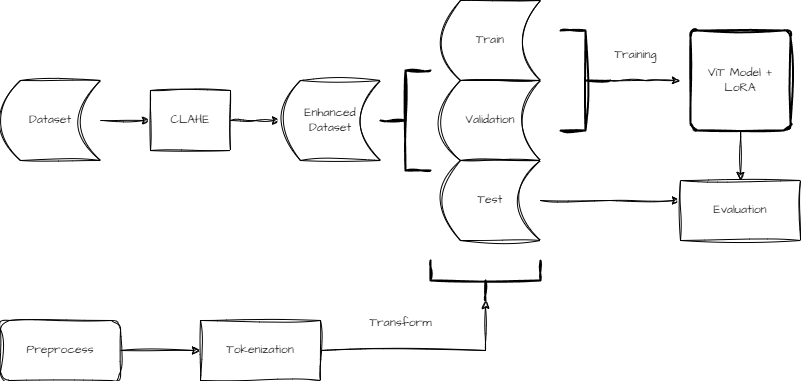
\includegraphics[width=1\linewidth]{breakhis.png}
    \caption{Workflow}
    \label{fig:enter-label}
\end{figure}

\subsection{Data Preparation}
We have to change the dataset to the Huggin Face dataset format for compatibility with the pre-trained model. Then we apply the CLAHE enhancement for the dataset. Images are converted to NumPy array which is better in computation then converted from RGB to LAB color space. After that, we control how much to limit contrast enhancement (avoids over-amplification) with rate clipLimit=2.0, images are divided into 8×8 tiles, histogram equalization is applied locally and merge enhanced L, A, and enhanced B together. Finally, we convert dataset back to RGB space.

Before tokenizing, we split the dataset into 70\% training, 10\% validation, and 20\% test to ensure effective model training, fine-tuning, and evaluation. Then we normalize images using normalization constants—mean: [0.485, 0.456, 0.406] and standard deviation: [0.229, 0.224, 0.225] of ImageNet dataset\cite{imagenet_cvpr09}. The next step is get images refined with resizing to (244, 244), horizontally flipping and converted to tensor format. The last step is using pre-trained transformer to transform data.

\subsection{Model}

We map labels to IDs with benign=0 and malignant=1. Then, we configure LoRA\cite{hu2022lora} with a rank of decomposition at 16, a scaling factor $\alpha$ at 16, and the target attention layers chosen as the query and value layers. The dropout rate is set to 0.1, and we keep the parameters for the classifier trainable. Finally, we train the fine-tuned model with a learning rate of $\mathbf{5 \times 10^{-3}}$ and 20 epochs.

\section{Result}
\subsection{Quantitive Result}
This model achieves significantly high result:
\begin{itemize}
    \setlength{\itemsep}{0pt}
    \item Accuracy: 0.9792418772563177.
    \item F1 Score: 0.9791851068309047.
    \item Precision: 0.9792189926509923.
    \item Recall": 0.9792418772563177.
\end{itemize}
\subsection{Qualitative Result}
The confusion matrix shows that there are only 50 cases in over 2300 test cases miss-classified (only 2.1\%).

\begin{figure}[H]
    \centering
    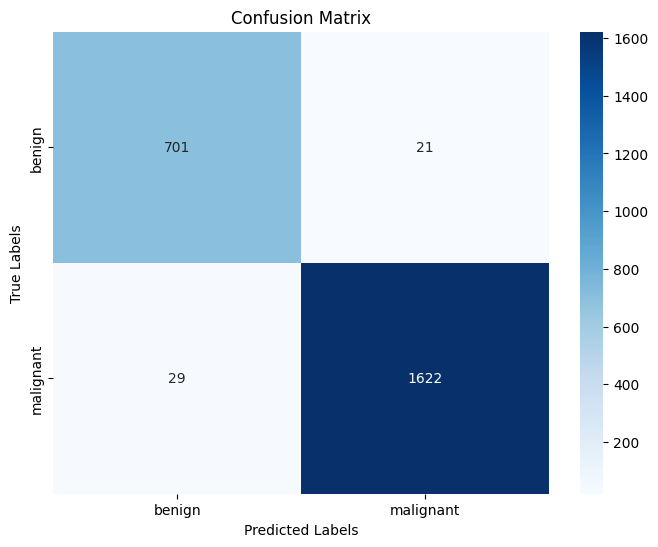
\includegraphics[width=1\linewidth]{confusion_matrix.png}
    \caption{Confusion Matrix}
    \label{fig:enter-label}
\end{figure}

\begin{figure}[H]
    \centering
    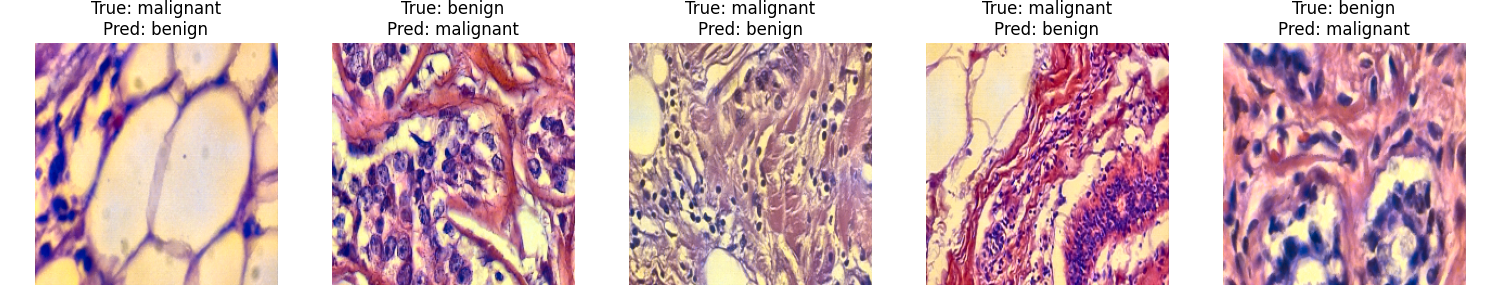
\includegraphics[width=1\linewidth]{wrong.png}
    \caption{Miss Classified Examples}
    \label{fig:enter-label}
\end{figure}

The learning curve also indicates that model is well-fitted and have magnificent performance on unseen data.

\begin{figure}[H]
    \centering
    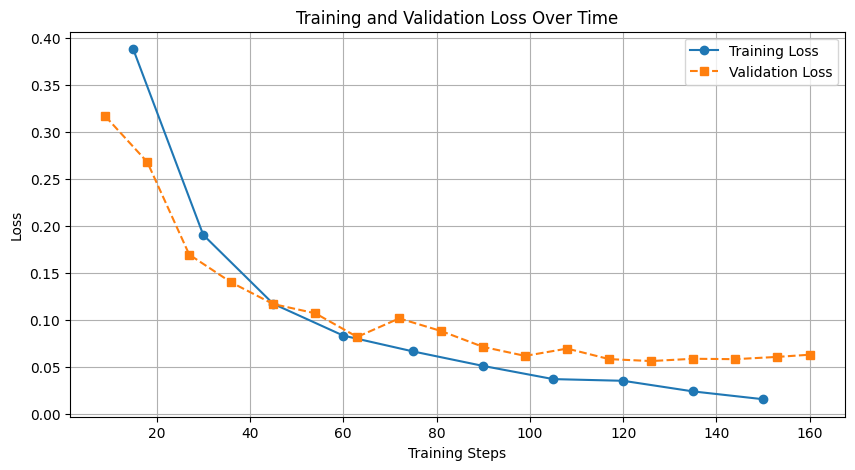
\includegraphics[width=1\linewidth]{loss.png}
    \caption{Training and Validation Loss overtime}
    \label{fig:enter-label}
\end{figure}

\section{Conclusion}
LoRA fine-tuning significantly improves performance while reducing computational cost by focusing on query and value attention layer that makes model achieves high accuracy \& F1-score, making it effective for breast cancer detection. Qualitative analysis shows the model focuses on meaningful features. 

\printbibliography
\addcontentsline{toc}{section}{References}

\end{document}